\documentclass[12pt]{article}
\usepackage{amsmath}
\usepackage{amssymb}
\usepackage{geometry}
\geometry{margin=1in}
\usepackage{tikz}

\begin{document}

\section*{Completing the square problems}

\begin{enumerate}
  \item Suppose the total area of the shape below is $40$. What is the value of $x$?
  
  \begin{center}
  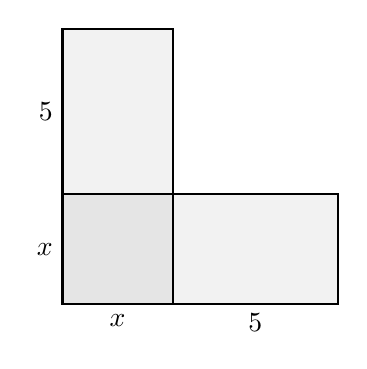
\begin{tikzpicture}[scale=0.7]
    % Draw the L-shape: x by x square (bottom left)
    \draw[thick,fill=gray!20] (0,0) rectangle (2,2);
    % x by 5 rectangle above x by x
    \draw[thick,fill=gray!10] (0,2) rectangle (2,5);
    % 5 by x rectangle to the right of x by x
    \draw[thick,fill=gray!10] (2,0) rectangle (5,2);
    % Outer L-shape boundary
    \draw[thick] (0,0) -- (0,5) -- (2,5) -- (2,2) -- (5,2) -- (5,0) -- cycle;
    % Dashed lines for clarity (optional, to show the grid)
    \draw[dashed] (2,0) -- (2,5);
    \draw[dashed] (0,2) -- (5,2);
    % Add 'x' and '5' labels
    % x by x square
    \node[below] at (1,0) {$x$};
    \node[left] at (0,1) {$x$};
    % x by 5 rectangle (above)
    \node[left] at (0,3.5) {$5$};
    % 5 by x rectangle (right)
    \node[below] at (3.5,0) {$5$};
  \end{tikzpicture}
  \end{center}

\end{enumerate}

\end{document} 